\begin{multicols}{2}
\subsubsection{Description}
\lipsum[1]
\subsubsection{Setup}

\textbf{Input:} Grayscale picture.\\
\textbf{Boundary conditions:} Fixed.\\
\textbf{Initial output:} Unimportant (all zeros)

\begin{minipage}{0.9\linewidth}
\begin{equation}
A =
\begin{bmatrix}
 0 & 0 & 0 \\
 0 & 0 & 0 \\
 0 & 0 & 0
\end{bmatrix}
B =
\begin{bmatrix}
 0 & 0 & 0 \\
 0 & 0 & 0 \\
 0 & 0 & 0
\end{bmatrix}
Z = 1
\end{equation}
\captionof{figure}{Chosen values of A,B and Z for this experiment}
\end{minipage}

\subsubsection{Results}


\begin{minipage}{0.5\linewidth}
	\centering
	
\includegraphics[width=0.9\linewidth]{./Experiments/Template/fig/1.png} 
	\captionof{figure}{Input}
\end{minipage}
\begin{minipage}{0.5\linewidth}
	\centering
	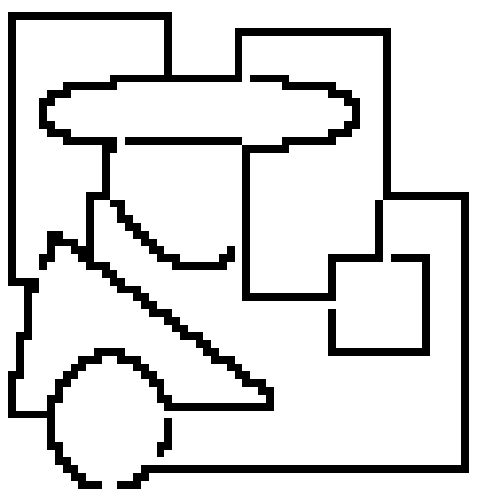
\includegraphics[width=0.9\linewidth]{./Experiments/Template/fig/2.png}
	\captionof{figure}{Output}
\end{minipage}

\lipsum[1]

\begin{minipage}{0.5\linewidth}
	\centering
	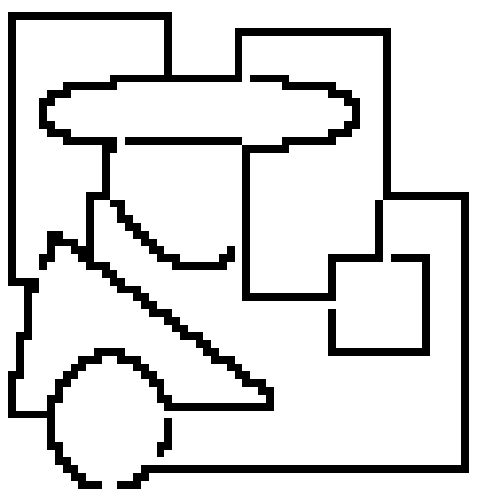
\includegraphics[width=0.9\linewidth]{./Experiments/Template/fig/2.png}
	\captionof{figure}{Alt1}
\end{minipage}
\begin{minipage}{0.5\linewidth}
	\centering
	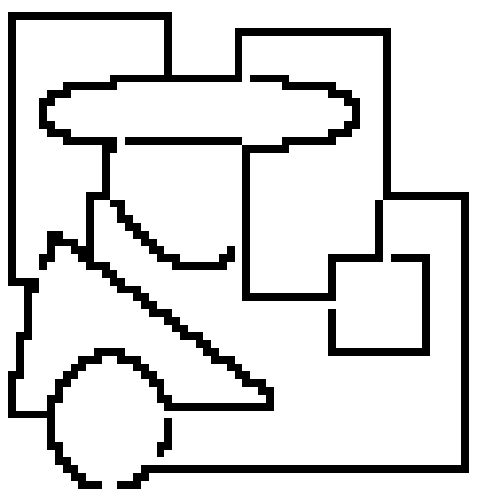
\includegraphics[width=0.9\linewidth]{./Experiments/Template/fig/2.png}
	\captionof{figure}{Alt2}
\end{minipage}
\begin{minipage}{0.5\linewidth}
	\centering
	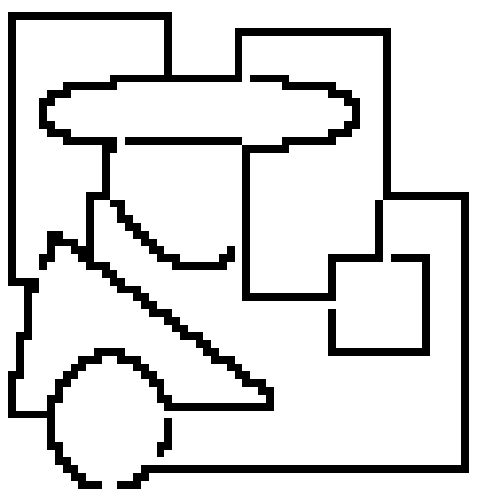
\includegraphics[width=0.9\linewidth]{./Experiments/Template/fig/2.png}
	\captionof{figure}{Alt3}
\end{minipage}
\begin{minipage}{0.5\linewidth}
	\centering
	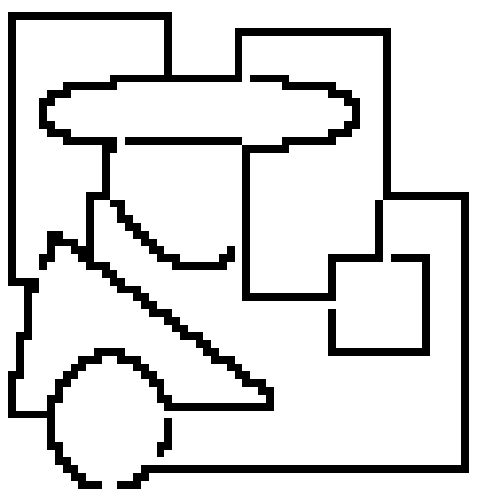
\includegraphics[width=0.9\linewidth]{./Experiments/Template/fig/2.png}
	\captionof{figure}{Alt4}
\end{minipage}
\lipsum[1]

\end{multicols}